\documentclass{article}
\usepackage{pdfpages}
\usepackage{verbatim}
\usepackage{csvsimple}


\begin{document}
	\begin{center}
		\begin{LARGE}
			\textbf{HW3}\\
		\end{LARGE}
		Yao, Yi\\
		sakfljklasdj
	\end{center}
	\begin{enumerate}
		\item 
		Application Introduction:\\
		This software simulates the operation of a north-south-one-lane bridge, whose capacity , as well as the north and south input buffers (queues) are in theory $+\infty$. When one side ends traversing the bridge, the other side starts traversing if cars are present in queue, otherwise, the same side starts traversing, if cars are present in queue. The model is implemented using Event Scheduling based Discrete Event Simulation.
		\item 
		Included is the file api.h:
		\verbatiminput{../src/engine/api.h}
		In this file that defines the api, there are function prototypes for creating the engine, scheduling events, starting simulation, generating random numbers and other utility functions.
		\item 
		\item 
		\item 
		Engine Introduction:\\
		The simulation engine implementation includes a future event list implemented with heap. The heapify up and heapify down functions are implemented with swapping the actual nodes.
		\item 
		Engine Testing Procedure:
		In order to make sure that the engine works, I wrote a trivial testing simulation.\\
		The testing program is in src/test\_app\\
		\verbatiminput{testpro.txt}
		The point starts at (0, 0). If the event type is 1, the new point is added to the point. If the type is 2, the new point is subtracted from the point.\\
		When an event is handled, an event will be scheduled at timestamp + 3 to subtract (1, 1)\\
		Here's the output from the test program:\\
		\verbatiminput{test.txt}
		From the output we can be sure that the behavior of the simulation engine is well defined.
		\item 
		Here's a sample output:\\
		\csvautotabular[respect all]{chk.csv}\\ \hfill \\
		North interarrival times have a mean of 50 seconds, while south interarrival times have a mean of 60 seconds.\\
		As is shown in the output, cars wait in queue when supposed to, traverse the bridge when supposed to and leaves the system when supposed to.
		\item 
		\begin{enumerate}
			\item 
			Below are plots from the experiments on the engine.\\
			The benchmark programs are in src/benchmark\\
			Using the scripts benchmark and benchmark1 in project root, experiments are done.
			The first experiment is done with initial events whose difference in timestamps exponentially distributed with mean 1. It is supposed to be close to what the application is doing.\\
			The results are in the first three plots. In the third plot, 1 represents data points from the heap representation. We can see that the heap implementation is actually slower than the list implementation. The reason might be that the insertion point is close to the head of the "list," giving the list implementation an advantage.\\
			The second experiment is done with initial points whose timestamps are uniformly distributed between 0 and 2\\
			The results are in plots 4 through 6. In the sixth plot, 1 represents data points from the heap implementation.
			Since the insertion point is far from the head, we can see a log growth in the heap implementation and a linear growth in the list implementation clearly in the plots, giving the heap implementation a huge advantage.\\
			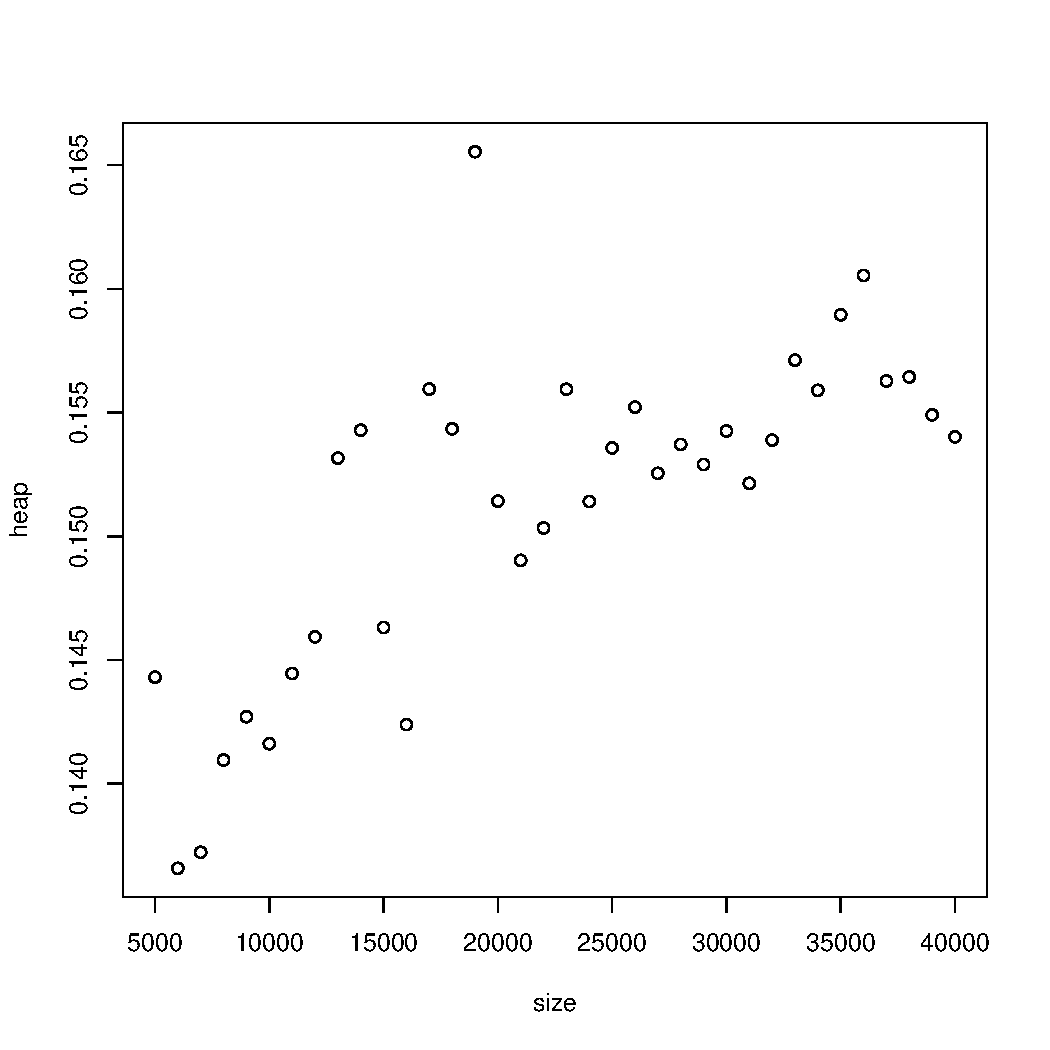
\includepdf[pages=-]{Rplots.pdf}
			\item 
			
		\end{enumerate}
		
	\end{enumerate}
	
	
	
\end{document}